\documentclass[12pt,letterpaper]{hmcpset}
\usepackage[margin=1in]{geometry}
\usepackage{graphicx}
\usepackage{enumitem} % enumerate
\newcommand{\ds}{\displaystyle}
% example usage of amssymb: $\mathbb{Z}$
% amsmath is loaded.

% info for header block in upper right hand corner
\name{}
\class{Math 19 - 07}
\assignment{Homework \#7}
\duedate{10/18/2019}

\begin{document}

\problemlist{Homework \#7}

\begin{problem}[1]
  \begin{enumerate}[label=(\alph*)]
  \item Compute the $(2n+1)$-order Taylor polynomial for $\sinh x$ using basepoint $x_0 = 0$. 
  \item Compute the $2n$-order Taylor polynomial for $\cosh x$ using basepoint  $x_0 = 0$. 
  \end{enumerate}
\end{problem}
\begin{solution}
\end{solution}
\pagebreak

\begin{problem}[2]
  The integral 
  \begin{equation}
    \int_a^b e^{-x^2} \, dx
    \label{int}
  \end{equation}
  is not directly computable since there is no known ``reasonable" function $F(x)$ with $F'(x) = e^{-x^2}$. This is an issue since integrals involving the Gaussian curve $e^{-x^2}$  are ubiquitous in statistics and science. In such cases, we can use Taylor polynomials to approximate the integrand and obtain estimates for the integral.  The general idea is 
  \[ f(x) \approx P(x) \implies \int_a^b f(x) \, dx \approx \int_a^b P(x) \, dx.  \]
  \begin{enumerate}[label=(\alph*)]
  \item Calculate the second-order Taylor polynomial for $e^{-x^2}$ for $x_0=0$. 
  \item Use your polynomial in (a)  to approximate the value of $\ds  \int_0^{0.25} e^{-x^2} \, dx$. 
  \item How does your estimate compare with a calculator estimate? 
  \end{enumerate}
\end{problem}
\begin{solution}
\end{solution}
\pagebreak
\begin{problem}[3]
  \phantom{first line of text} \\
  \parbox{0.5\textwidth}{
    \vspace{\baselineskip}
    Consider a general triangle with side lengths $a, b$, and $c$, as in the figure. In this exercise we will prove the \textit{Law of Cosines}:
    \begin{equation}
      c^2 = a^2 + b^2 - 2 a b \cos \theta
      \label{lc}
    \end{equation}
    (when $\theta = \frac{\pi}{2}$ this agrees with the Pythagorean Theorem). 
    Begin your proof by applying the Pythagorean theorem to the right triangle with hypotenuse $c$.
    Note that for the right triangle with hypotenuse $b$ we know  $x=b \cos \theta $ and $y = b \sin \theta$.
  }
  \parbox{0.5\textwidth}{
    \[ 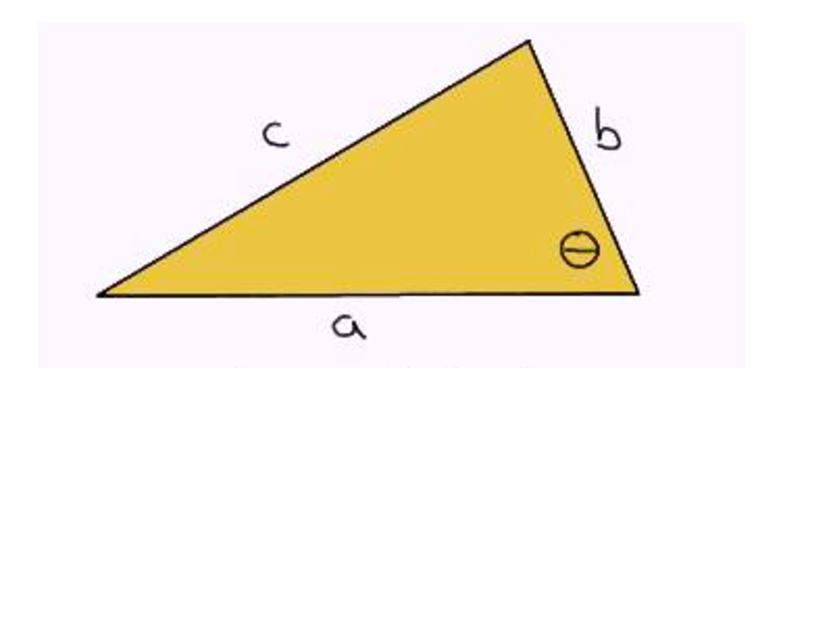
\includegraphics[width=0.325\textwidth]{assets/Lawcos2} \]
    \[ 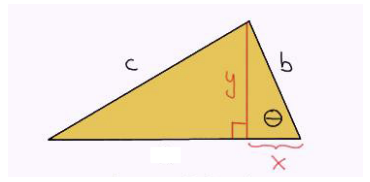
\includegraphics[width=0.325\textwidth]{assets/Lawcos1b2} \]
  }
\end{problem}
\begin{solution}
\end{solution}
\pagebreak

\begin{problem}[4]
  \begin{enumerate}[label=(\alph*)]
  \item Read Colley Section 1.3. Explain the meaning of $\text{proj}_{\mathbf{a}} \mathbf{b}$
    to any friend (in Math 19 or not). Write down the name of this friend for your solution to Part (a).
  \item Determine $\text{proj}_{\mathbf{a}} \mathbf{b}$ for $\mathbf{a} = (0,1,0)$ and
    $\mathbf{b} = (2,3,4)$.
  \item Provide a solution for Exercise 1.3.24 in Colley (Suppose that a force $\mathbf{F} = \mathbf{i} - 2 \mathbf{j}$\dots). \\
    
    \textbf{Colley 1.3.24: } Suppose that a force $\mathbf{F} = \mathbf{i} - 2\mathbf{j}$ is acting on an object moving parallel to the vector $\mathbf{a} = 4\mathbf{i} + \mathbf{j}$. Decompose $\mathbf{F}$ into a sum of vectors $\mathbf{F}_1$ and $\mathbf{F}_2$, where $\mathbf{F}_1$ points along the direction of motion and $\mathbf{F}_2$ is perpendicular to the direction of motion. (Hint: A diagram may help.)
  \end{enumerate}
\end{problem}

\end{document}
